% !TeX program = xelatex
\documentclass[11pt,a4paper]{article}
\usepackage[UTF8,scheme=plain,fontset=windows]{ctex}
\usepackage{amsmath,amssymb,amsthm,bm}
\usepackage[a4paper,margin=25mm]{geometry}
\usepackage{graphicx,booktabs,tabularx,array,longtable,multirow}
\usepackage{algorithm,algpseudocode}
\usepackage{tikz}
\usetikzlibrary{arrows.meta,positioning,fit}
\usepackage{caption,subcaption,placeins,needspace}
\usepackage[numbers,sort&compress]{natbib}
\usepackage[unicode,hidelinks]{hyperref}
\numberwithin{equation}{section}
\numberwithin{figure}{section}
\numberwithin{table}{section}
\newtheorem{proposition}{命题}[section]
\newtheorem{corollary}[proposition]{推论}
\renewcommand{\proofname}{证明}
\renewcommand{\figurename}{图}
\renewcommand{\tablename}{表}
\renewcommand{\abstractname}{摘要}
\floatname{algorithm}{算法}
\algrenewcommand{\algorithmicrequire}{\textbf{输入：}}
\renewcommand{\refname}{参考文献}
\newcommand{\R}{\mathbb R}
\newcommand{\C}{\mathbb C}
\newcommand{\E}{\mathbb E}
\newcommand{\Rea}{\operatorname{Re}}
\newcommand{\tr}{\operatorname{tr}}
\newcommand{\diag}{\operatorname{diag}}
\newcommand{\pending}[1]{\par\smallskip\noindent\fbox{\parbox{.94\linewidth}{\small 初稿待补：#1}}\par\smallskip}
\setlength{\parindent}{2em}
\setlength{\parskip}{.15em}
\setlength{\emergencystretch}{2em}
\linespread{1.15}
\captionsetup{font=small,labelfont=bf,labelsep=quad}
\raggedbottom
\renewcommand{\topfraction}{.9}
\renewcommand{\textfraction}{.05}
\renewcommand{\floatpagefraction}{.85}
\makeatletter
\renewcommand{\maketitle}{\begin{center}\LARGE\bfseries\@title\par\end{center}\vspace{.5em}}
\setlength{\@fptop}{0pt}
\setlength{\@fpsep}{18pt plus 2pt minus 2pt}
\makeatother
\title{\bfseries 未知宽带强弱重叠源的高效直接定位：\\多候选联合精修与波形消元更新}
\author{}
\date{}
\begin{document}
\maketitle
\begin{abstract}
多个同步单天线接收站对未知宽带波形进行直接定位时，频谱重叠与功率不平衡使位置搜索和信号估计相互耦合。单源空间谱的高分位置未必构成有效的多源解，逐源更新也可能因反复估计信号系数而缓慢收敛。本文在已知自由空间相对幅度与基带时延模型下，以最小二乘消去未知波形，建立统一的位置目标，并提出两种求解策略。多候选联合精修AP保留条件谱中的少量局部极大值，对各分支联合优化位置，再按拟合残差择优；波形消元块NOMP在残差发现和循环更新中使用消元后的局部位置目标，减轻固定信号系数对位置步长的约束。通过推导条件投影与消元曲率，本文解释两种策略的作用，并以配对实验检验其精度与计算成本。已完成的120条双源观测中，多候选联合AP恢复了单候选遗漏的10条观测；在相同停止精度下，单候选联合精修的平均求解时间比交替精修减少约8.2\%。八条观测的受控机制实验进一步表明，消元更新能显著减少固定系数更新的重复计算。候选保留与波形消元分别从搜索可靠性和更新效率改善了该模型下的直接定位。
\end{abstract}
\noindent\textbf{关键词：}直接位置估计；强弱重叠源；交替投影；块NOMP；可分离非线性最小二乘

\section{引言}\label{sec:introduction}
辐射源定位常先估计到达时间差等中间量，再由这些量求解位置。广义互相关与双曲线定位为这一流程提供了成熟工具\cite{KnappCarter1976,ChanHo1994}。当多个源使用重叠频带且波形未知时，各站接收的是不同传播响应下的混合信号，中间量的提取与跨站关联随之变难。直接位置估计（direct position determination，DPD）将传播关系直接带入观测模型，以位置作为主要待估参数，为多源联合处理提供了另一条途径\cite{ChenHudsonYao2002,WeissAmar2005}。

本文关注四个同步单天线站接收两个独立宽带源的情形。两源中心频率和带宽相同，接收功率可以明显不同，发射波形与发射功率未知。各站满足同一确定性传播规律，待解决的是如何从一次有限时长观测中高效求出两个位置。对这一问题，仅在单源谱中取两个峰容易把强源的邻峰当作第二个源；直接对两个二维位置做全网格组合搜索，又需要与网格点数平方成正比的计算。即使采用逐源求解，候选进入哪个局部区域、局部更新时是否重新估计波形，也会影响精度和成本。

宽带最大似然与交替投影（alternating projection，AP）通过固定部分位置、更新其余位置来降低联合搜索的维数\cite{ChenHudsonYao2002}。MUSIC型DPD利用噪声子空间检验位置响应\cite{WeissAmar2005}，MVDR借助协方差逆矩阵形成抑制干扰的空间评分\cite{Capon1969}；DPD-HR进一步研究了MVDR思想下的直接定位\cite{TirerWeiss2016}。这些准则依赖不同的观测与统计条件，比较时需要统一有效频带、传播信息和输入样本。

稀疏参数估计将粗搜索与离网精修结合起来。Newtonized orthogonal matching pursuit（NOMP）在贪心发现后进行Newton更新和循环精修\cite{Mamandipoor2016}。多频率二维块NOMP已用于离网波束形成\cite{Yang2022}；QNOMP采用准Newton联合优化改善多径参数估计\cite{Zeng2025}。这些研究已涵盖多频率建模、二维精修和联合优化。本文关注未知宽带波形怎样消元、强弱源候选怎样保留，以及这些选择如何影响实际定位成本。

可分离非线性最小二乘的变量投影思想，可将线性系数从非线性参数优化中消去\cite{GolubPereyra1973}。在本文场景中，位置为非线性参数，每个频点的源信号系数为线性参数。若局部位置试探仍使用固定的信号系数，所见曲率会包含本可由信号重估吸收的变化。另一方面，粗条件谱的排序并不保证精修后的排序。前者影响更新效率，后者影响可到达的解，因而需要分别处理。

围绕这些问题，本文形成以下三项工作。
\begin{enumerate}
  \item 针对同步单天线站的未知宽带强弱重叠源定位，建立统一的基带观测、功率与波形消元模型，将逐源发现、条件搜索及联合精修写在同一最小二乘目标下，明确不同求解策略的关系。
  \item 提出多候选联合精修AP：保留少量条件候选，联合调整源位置并重估波形，以精修后的目标选择分支。给出条件投影与联合拟合的等价关系，分析候选保留和联合更新分别承担的作用。
  \item 提出波形消元块NOMP：保留残差发现与循环更新，改用消元后的局部位置目标。通过Schur补刻画固定系数与消元曲率的差别，并结合受控对照和运算计数分析其计算优势。
\end{enumerate}

下文给出统一模型、两种求解算法及其计算关系，随后以基线比较、候选拆分和受控实验检验方法效果。扩大布局的比较沿用相同模型与评价口径，汇总结果经核验后纳入最终稿。

\section{观测模型与定位目标}\label{sec:model}
\subsection{同步单天线站的宽带观测}
设$L$个站的已知位置为$\bm r_l\in\R^2$，$K$个源的未知位置为$\bm p_k\in\Omega\subset\R^2$。记
\begin{equation}
 d_{lk}=\|\bm p_k-\bm r_l\|_2,\qquad
 \tau_{lk}=d_{lk}/c_0,\qquad \beta_{lk}=d_{lk}^{-1},
 \label{eq:distance}
\end{equation}
其中$c_0$为传播速度。各站时间、频率及接收链路同步，发射天线各向一致。幅度采用自由空间$1/d$规律；固定工作条件下的公共比例系数并入源波形。时移与相位从基带出发建模。于是
\begin{equation}
 x_l[n]=\sum_{k=1}^{K}\beta_{lk}s_k(n/f_s-\tau_{lk})+w_l[n],
 \quad n=0,\ldots,N-1 .\label{eq:time}
\end{equation}
源波形$s_k(t)$互相独立且未知，其幅度包含未知发射功率。噪声$w_l[n]\sim\mathcal{CN}(0,\sigma_t^2)$，在站间和采样点间独立。本模型中，每给定一个候选位置，其跨站相对响应即可计算。

将各站记录作$1/N$归一化DFT，保留公共处理频带$\mathcal F$。在共同观测窗的频域时延表示下，令
\begin{align}
 \bm x_f&=\bm A_f(\bm P)\bm s_f+\bm n_f,\quad f\in\mathcal F,\label{eq:frequency}\\
 [\bm a_f(\bm p)]_l&=\frac{1}{d_l(\bm p)}
       \exp[-\mathrm j2\pi f d_l(\bm p)/c_0],\label{eq:response}\\
 \bm A_f(\bm P)&=[\bm a_f(\bm p_1),\ldots,\bm a_f(\bm p_K)],\quad
 \bm P=[\bm p_1,\ldots,\bm p_K].\nonumber
\end{align}
此处$f$为带符号的基带频率，$F=|\mathcal F|$。波形经连续时延后在有限窗内采样，频域模型相应采用共同窗下的时延近似。噪声在所选DFT频点上的方差仍为$\sigma_t^2/N$，频点筛选保留原DFT归一化分母。

计算中也可用单位范数列$\bm q_f(\bm p)=\bm a_f(\bm p)/\|\bm a_f(\bm p)\|_2$。当逐频源系数自由估计时，列缩放不改变$\bm A_f$的列空间，因此不改变消元目标。它仍保留同一源在不同站之间的相对幅度。

\subsection{带内信噪比与强弱源条件}
记第$k$个源在第$l$站的时间平均接收功率为$P_{lk}$。名义信号带宽为$B$，白噪声在该带内的期望功率为$\sigma_t^2B/f_s$。本文采用
\begin{equation}
 \mathrm{SNR}_{k,\mathrm{in}}
 =10\log_{10}\frac{L^{-1}\sum_{l=1}^L P_{lk}}
 {\sigma_t^2B/f_s},\qquad
 \Delta=10\log_{10}\frac{\sum_l P_{l1}}{\sum_l P_{l2}} .
 \label{eq:snr}
\end{equation}
实验固定源2的波形、功率和噪声，仅缩放源1。$\Delta>0$时称源1为强源、源2为弱源；$\Delta=0$时保留这两个身份编号。各站局部功率差随几何变化，不强制等于四站平均的$\Delta$。

\subsection{未知波形消元与联合位置估计}
在白噪声模型下，将逐频未知信号作为确定性待估系数，可得到最小二乘位置准则。以观测总能量$E_x=\sum_f\|\bm x_f\|_2^2$归一化，定义
\begin{align}
 \mathcal L(\bm P,\{\bm s_f\})
   &=E_x^{-1}\sum_f\|\bm x_f-\bm A_f(\bm P)\bm s_f\|_2^2,\label{eq:fullLS}\\
 \widehat{\bm s}_f(\bm P)&=\bm A_f(\bm P)^\dagger\bm x_f,\label{eq:waveLS}\\
 J(\bm P)&=E_x^{-1}\sum_f\|\bm\Pi_{\bm A_f}^{\perp}\bm x_f\|_2^2,
 \quad \bm\Pi_{\bm A_f}^{\perp}=\bm I-\bm A_f\bm A_f^\dagger .\label{eq:profile}
\end{align}
所求位置为$\widehat{\bm P}=\arg\min_{\bm P\in\Omega^K}J(\bm P)$。对于本文的$K=2$，这是四维位置优化。不同源的系数在每次位置试探时共同重估，故$J$描述的是两个位置对原始混合观测的联合解释。

单源最小二乘谱则为
\begin{equation}
 Q_0(\bm p)=E_x^{-1}\sum_f
 \frac{|\bm a_f(\bm p)^H\bm x_f|^2}{\|\bm a_f(\bm p)\|_2^2} .\label{eq:single}
\end{equation}
单源情形下，最大化$Q_0$与最小化$J$等价；从同一张$Q_0$中直接取两个峰，则没有显式拟合两源之间的相互影响。这一区别是后续多源算法设计的起点。

\section{多候选联合AP与波形消元块NOMP}\label{sec:methods}
\subsection{条件投影搜索}
给定其他源的位置，将其响应组成$\bm B_f$。令
\begin{equation}
 \bm r_f=\bm\Pi_{\bm B_f}^{\perp}\bm x_f,\qquad
 \bm u_f(\bm p)=\bm\Pi_{\bm B_f}^{\perp}\bm a_f(\bm p).
\end{equation}
条件位置谱为
\begin{equation}
 Q_{\mathrm{AP}}(\bm p\mid\bm B)
 =E_x^{-1}\sum_f\frac{|\bm u_f(\bm p)^H\bm r_f|^2}
 {\|\bm u_f(\bm p)\|_2^2}.\label{eq:conditional}
\end{equation}
若$\bm u_f=0$，该频点新增位置不扩展已有列空间，其贡献记为零。

\begin{proposition}[条件谱与联合残差]\label{prop:conditional}
固定$\bm B_f$时，在每个频点共同重估原有源与新源的系数，增加候选$\bm a_f(\bm p)$带来的归一化最小残差下降量恰为式\eqref{eq:conditional}。
\end{proposition}
\begin{proof}
将$\bm a_f$分解为其在$\operatorname{col}(\bm B_f)$中的分量与正交分量$\bm u_f$。当$\bm u_f\ne0$时，新增列空间的投影为$\bm u_f\bm u_f^H/\|\bm u_f\|^2$，与$\bm B_f$的投影正交。因此
\begin{equation}
 \bm\Pi_{[\bm B_f,\bm a_f]}^{\perp}
 =\bm\Pi_{\bm B_f}^{\perp}
 -\frac{\bm u_f\bm u_f^H}{\|\bm u_f\|^2} .
\end{equation}
以$\bm x_f$左右相乘并对频点求和，即得所述残差下降量。零正交分量的情形由列空间不变直接得到。
\end{proof}

式\eqref{eq:conditional}不仅把已发现源的贡献从观测中投影掉，也对新位置的响应作同一投影。这使条件搜索与式\eqref{eq:profile}保持一致。它沿用AP的条件优化思想\cite{ChenHudsonYao2002}，为下面的候选分支提供统一评分。

\subsection{多候选联合精修AP（MCJ-AP）}\label{sec:mcj}
先在公共粗网格$\mathcal G$上最大化$Q_0$，并作单源连续精修，得到$\bm p_1^{(0)}$。固定此位置，计算第二源条件谱，保留$M$个相互分离的局部极大值$\bm c_1,\ldots,\bm c_M$。每个初始组合$[\bm p_1^{(0)},\bm c_m]$进入同一个联合位置目标：
\begin{equation}
 \widehat{\bm P}^{(m)}=\operatorname{LocalMin}_{\bm P\in\Omega^2}
 J(\bm P;[\bm p_1^{(0)},\bm c_m]),\qquad
 m^*=\arg\min_m J(\widehat{\bm P}^{(m)}).\label{eq:branch}
\end{equation}
最终输出$\widehat{\bm P}^{(m^*)}$。分支选择只使用混合观测的拟合目标，不使用真实位置、真实频带或真实源波形。

\begin{algorithm}[H]
\caption{多候选联合精修AP}\label{alg:ap}
\begin{algorithmic}[1]
\Require 观测$\{\bm x_f\}$，站点坐标，公共网格$\mathcal G$，候选数$M$
\State 最大化$Q_0$并单源精修，得到$\bm p_1^{(0)}$
\State 固定$\bm p_1^{(0)}$，以式\eqref{eq:conditional}扫描$\mathcal G$
\State 按固定局部极大值与间距规则保留$M$个候选
\For{$m=1,\ldots,M$}
  \State 从$[\bm p_1^{(0)},\bm c_m]$联合优化$J$；每次试探按式\eqref{eq:waveLS}重估波形
  \State 保存该分支的目标、位置与停止状态
\EndFor
\State 按式\eqref{eq:branch}输出最小残差分支
\end{algorithmic}
\end{algorithm}

采用L-BFGS-B处理搜索边界\cite{Byrd1995}。记$\bm e_f=\bm x_f-\bm A_f\widehat{\bm s}_f$，由最小二乘正交条件$\bm A_f^H\bm e_f=0$，位置梯度为
\begin{equation}
 \frac{\partial J}{\partial\theta_i}
 =-\frac{2}{E_x}\Rea\sum_f
 \bm e_f^H\frac{\partial\bm A_f}{\partial\theta_i}
 \widehat{\bm s}_f,\label{eq:gradient}
\end{equation}
其中$\bm\theta=\operatorname{vec}(\bm P)$。对$\bm v_l=(\bm p-\bm r_l)/d_l$，响应导数为
\begin{equation}
 \nabla_{\bm p}a_l(f,\bm p)
 =a_l(f,\bm p)\left(-\frac1{d_l}-\mathrm j\frac{2\pi f}{c_0}\right)\bm v_l.
 \label{eq:responseDerivative}
\end{equation}
式\eqref{eq:gradient}无需显式求出波形估计对位置的导数，减少了联合优化中的计算与实现负担。

\begin{proposition}[嵌套候选的目标关系]\label{prop:branches}
若两个候选集合嵌套，公共分支采用相同初始化、确定性求解器和停止条件，则增加候选后所选解的$J$不增。
\end{proposition}
\begin{proof}
小候选集的全部精修结果仍属于大候选集的可选结果，对更大集合取最小值不大于对子集取最小值。
\end{proof}
保留候选扩大了精修后可供择优的解集。位置精度还受噪声与局部目标结构影响，实验因此同时报告位置误差和拟合残差。$M=1$为轻量版本；$M>1$用于比较额外分支带来的可靠性与成本。

\subsection{波形消元块NOMP（VP-BNOMP）}\label{sec:vpnomp}
NOMP通过残差发现新成分，并循环修正已发现参数\cite{Mamandipoor2016}。二维多频率块NOMP将每个位置对应的逐频系数作为一个块\cite{Yang2022}。本文保留这一发现和循环结构，把局部位置更新写成消元最小二乘问题。

给定当前位置和共同系数估计，更新源$j$时构造
\begin{equation}
 \bm y_{j,f}=\bm x_f-\sum_{k\ne j}\bm a_f(\bm p_k)\widehat s_{k,f} .
 \label{eq:targetResidual}
\end{equation}
局部试探位置$\bm p$对应的最优系数与目标分别为
\begin{align}
 \widehat q_f(\bm p)&=\frac{\bm a_f(\bm p)^H\bm y_{j,f}}
 {\|\bm a_f(\bm p)\|^2},\label{eq:localcoef}\\
 \phi_j(\bm p)&=\min_{\{q_f\}}E_x^{-1}\sum_f
 \|\bm y_{j,f}-\bm a_f(\bm p)q_f\|^2\nonumber\\
 &=E_x^{-1}\sum_f\left(\|\bm y_{j,f}\|^2-
 \frac{|\bm a_f(\bm p)^H\bm y_{j,f}|^2}{\|\bm a_f(\bm p)\|^2}\right).
 \label{eq:localprofile}
\end{align}
Newton更新使用$\phi_j$的位置梯度和Hessian，而非将$q_f$固定后的曲率。执行有界步长和回溯后，以完整$J$检查接受条件；接受位置后共同重估全部源系数。残差发现使用
\begin{equation}
 Q_{\mathrm R}(\bm p)=E_x^{-1}\sum_f
 \frac{|\bm a_f(\bm p)^H\bm r_f|^2}{\|\bm a_f(\bm p)\|^2},
 \label{eq:residualScore}
\end{equation}
其中$\bm r_f$为当前共同拟合的残差。

\begin{algorithm}[H]
\caption{波形消元块NOMP}\label{alg:nomp}
\begin{algorithmic}[1]
\Require 观测，公共网格，源数$K$，循环与Newton停止参数
\State 初始化源集合为空，$\bm r_f\gets\bm x_f$
\For{$k=1,\ldots,K$}
  \State 最大化残差谱\eqref{eq:residualScore}，发现新位置
  \State 以式\eqref{eq:localprofile}作单源Newton精修，加入源集合
  \State 按式\eqref{eq:waveLS}共同重估全部已发现源的系数
  \Repeat
    \For{已发现的每个源$j$}
      \State 构造$\bm y_{j,f}$，用$\phi_j$作有界Newton更新
      \State 仅接受使完整$J$不增的位置，并共同重估系数
    \EndFor
  \Until{循环停止条件满足或达到安全上限}
  \State 更新共同拟合残差
\EndFor
\State 输出已发现位置；可单列末端联合精修版本用于比较
\end{algorithmic}
\end{algorithm}

AP的条件谱和NOMP的残差谱并不相同。对单个频点，因$\bm r_f\perp\operatorname{col}(\bm B_f)$，二者分子相同，而分母分别为$\|\bm\Pi_{\bm B_f}^{\perp}\bm a_f\|^2$和$\|\bm a_f\|^2$。因此，它们可能发现不同的初始区域。本文保留各自的发现机制，而非用AP的搜索替换NOMP。

\subsection{消元更新的曲率与下降性质}\label{sec:curvature}
将复信号系数的实部、虚部写为实向量$\bm u$，位置写为$\bm z$。局部损失记作$L(\bm z,\bm u)$，$\widehat{\bm u}(\bm z)$为给定位置的最小二乘解。
\begin{proposition}[消元曲率]\label{prop:schur}
在响应可微且系数最小二乘解局部唯一的区域，令$\varphi(\bm z)=L(\bm z,\widehat{\bm u}(\bm z))$，则
\begin{align}
 \nabla\varphi&=L_{\bm z},\label{eq:envelope}\\
 H_{\mathrm{VP}}&=H_{zz}-H_{zu}H_{uu}^{-1}H_{uz},\label{eq:schur}\\
 H_{zz}-H_{\mathrm{VP}}&\succeq0 .\label{eq:psd}
\end{align}
所有偏导均在$(\bm z,\widehat{\bm u}(\bm z))$处取值。
\end{proposition}
\begin{proof}
最小二乘一阶条件为$L_{\bm u}=0$。对$\bm z$求导，有$\partial\widehat{\bm u}/\partial\bm z=-H_{uu}^{-1}H_{uz}$。代入$\varphi$的一、二阶导数得到式\eqref{eq:envelope}和\eqref{eq:schur}。系数子问题的$H_{uu}$正定，故$H_{zu}H_{uu}^{-1}H_{uz}$半正定。
\end{proof}

命题\ref{prop:schur}揭示了固定系数更新缓慢的一种机制。固定系数Hessian保留了波形重估本可吸收的响应变化，在位置--系数耦合较强的方向上可能偏大，从而缩短位置步长。消元更新扣除这一项。本文依据变量投影原理\cite{GolubPereyra1973}构造逐源宽带位置更新，并通过只改变局部目标的对照检验其作用。

更具体地，在局部极小点附近，若$H_{zz}$和$H_{\mathrm{VP}}$均正定，用固定系数曲率更新消元梯度，其一阶误差传播为
\begin{equation}
 \bm e^{+}\approx
 \left(\bm I-H_{zz}^{-1}H_{\mathrm{VP}}\right)\bm e .\label{eq:localrate}
\end{equation}
式\eqref{eq:psd}使该迭代矩阵的特征值落在$[0,1)$。当消元曲率相对固定系数曲率很小时，部分方向的收缩因子接近1，表现为大量小步更新。使用精确消元Newton曲率，则去掉了这一局部线性误差项。数值保护、线搜索及近似Hessian仍会影响实测迭代次数。

联合位置精修处理的是另一层耦合。双源位置Hessian含有非零的跨源块$H_{12}$：
\begin{equation}
 H_{\mathrm{joint}}=
 \begin{bmatrix}H_{11}&H_{12}\\H_{21}&H_{22}\end{bmatrix} .
\end{equation}
逐源精修固定另一位置，联合精修同时利用两个位置方向的信息。MCJ-AP采用联合L-BFGS-B近似这一关系；VP-BNOMP首先改善每个源内部的位置--系数耦合，末端联合位置精修作为独立变体比较。

\begin{proposition}[已接受目标的单调性]
若每次更新仅接受$J(\bm P^{+})\le J(\bm P)$的位置，则已接受目标序列收敛。
\end{proposition}
\begin{proof}
由式\eqref{eq:profile}，$J\ge0$。已接受目标单调不增且有下界，故收敛。
\end{proof}
目标下降检验使迭代保持稳定，候选发现决定进入的搜索区域，安全上限控制计算预算；三者共同构成求解流程。

\subsection{计算量及方法关系}\label{sec:complexity}
令$G$为网格点数，$I$为循环次数，$T$为连续目标与梯度的调用次数。单次联合系数求解需要形成$K\times K$ Gram矩阵，其主要计算量为$\mathcal O(F(LK^2+K^3))$。固定其他源的投影可预计算，条件网格扫描主要为$\mathcal O(FGLK)$。双源全组合网格需$G^2$组位置，而两次条件或残差扫描随$G$线性增长。

\begin{table}[t]
\centering\small
\caption{主要计算量。$I_{\mathrm B}$为稀疏贝叶斯迭代数，$S$为分段数。}\label{tab:complexity}
\begin{tabularx}{\linewidth}{@{}lX@{}}\toprule
方法或运算 & 主要量级与可观测计数\\\midrule
公共DFT & $\mathcal O(LN\log N)$；原始采样点与保留频点数\\
MUSIC／MVDR & 统计约$\mathcal O(F_sSL^2+F_sL^3)$，谱扫描$\mathcal O(F_sGL^2)$；$F_s$为分段后频点数\\
MCJ-AP & 两次条件扫描加$M$个局部位置优化；约$\mathcal O(FGLK+T_MF(LK^2+K^3))$\\
VP-BNOMP & 逐源扫描与$I$轮循环精修；约$\mathcal O(KFGL+IKT_{\mathrm{loc}}FL)$，另计共同系数重估\\
多初值／GA & 由位置目标调用总数$T$决定，约$\mathcal O(TF(LK^2+K^3))$\\
宽带SBL & 稠密字典每轮约$\mathcal O(FGL^2+FL^3)$，累计随$I_{\mathrm B}$增长\\\bottomrule
\end{tabularx}
\end{table}
本文的计算改进主要体现在减少调用次数，而非改变所有运算的渐近阶数。表中分支调用数覆盖全部候选，局部调用数对应单次源位置更新。局部单源系数按频点独立，式\eqref{eq:schur}的系数块仅为逐频$2\times2$实矩阵；累加后得到$2\times2$位置曲率，无需构造$2F\times2F$矩阵。固定系数与消元更新都可按$F$线性计算，效率差别由曲率质量与实际循环数体现。表\ref{tab:complexity}因此与实验中的扫描点数、目标/梯度调用数和完整耗时对应报告。

AP、NOMP、BNOMP与QNOMP分别提供条件搜索、残差发现、块更新与联合准Newton优化的研究基础\cite{ChenHudsonYao2002,Mamandipoor2016,Yang2022,Zeng2025}。本文方法的重点是：在同一未知波形直接定位模型中，明确候选保留、系数消元和联合位置精修的职责，并用控制变量实验建立这些选择与定位成本之间的联系。

\section{仿真实验}\label{sec:experiments}
\subsection{场景与实验组织}
四站坐标分别为$(500,0)$、$(0,500)$、$(-500,0)$和$(0,-500)$\,m，最大基线$R=1000$\,m。搜索区域为$[-1000,1000]^2$\,m$^2$，源位置为连续坐标。表\ref{tab:scenario}给出公共信号设置。两源的符号、波形初相与定时独立，同一次基础实现的六档功率差共享波形和噪声，仅缩放源1。

\begin{table}[htbp]\centering\small
\caption{公共仿真参数。}\label{tab:scenario}
\begin{tabularx}{.95\linewidth}{@{}lX@{}}\toprule
参数 & 设置\\\midrule
接收站／源数 & 四个同步单天线站；已知$K=2$\\
传播 & 自由空间相对幅度$1/d$与基带时延；$c_0=3\times10^8$\,m/s\\
波形 & 独立BPSK，根升余弦脉冲，符号率10\,MHz，滚降0.25\\
中心与名义带宽 & 两源中心均为0；带宽均为12.5\,MHz\\
采样与记录 & 50\,MHz；8192点；163.84\,$\mu$s\\
处理频带 & $[-7,7]$\,MHz；完整记录DFT保留2293个频点\\
噪声与信噪比 & 时域复噪声方差1；弱源四站平均带内SNR为6\,dB\\
平均接收功率差 & 0、3、6、9、12、15\,dB\\
初始网格 & 各方法统一20\,m，$101\times101=10201$个点\\
连续精修与输出 & 保留各方法原生精修；已知源数，不使用真实源身份排序\\\bottomrule
\end{tabularx}
\end{table}

已完成实验包含三组互补证据。第一组比较公共带限输入下的定位方法，并配套孤立弱源、孤立强源观测，用来区分单源可定位性和混合损失。第二组使用新的四类布局、每布局五次随机实现，共120条混合观测，对候选和精修作配对比较；随后在同一批观测上补充五候选AP。第三组复用八条观测，对固定系数更新与消元更新进行受控机制比较。不同组使用各自登记的实现，不将它们拼成同一独立样本总体。

图\ref{fig:geometry}给出第二组的四个布局。站内指四站凸包内部；站外仍位于搜索区域内。几何生成时排除距任一站小于150\,m、距布局中心小于100\,m、距站点对连线小于50\,m的位置，双源间距至少300\,m。坐标由几何规则确定，不按定位结果选择。
\begin{figure}[htbp]\centering
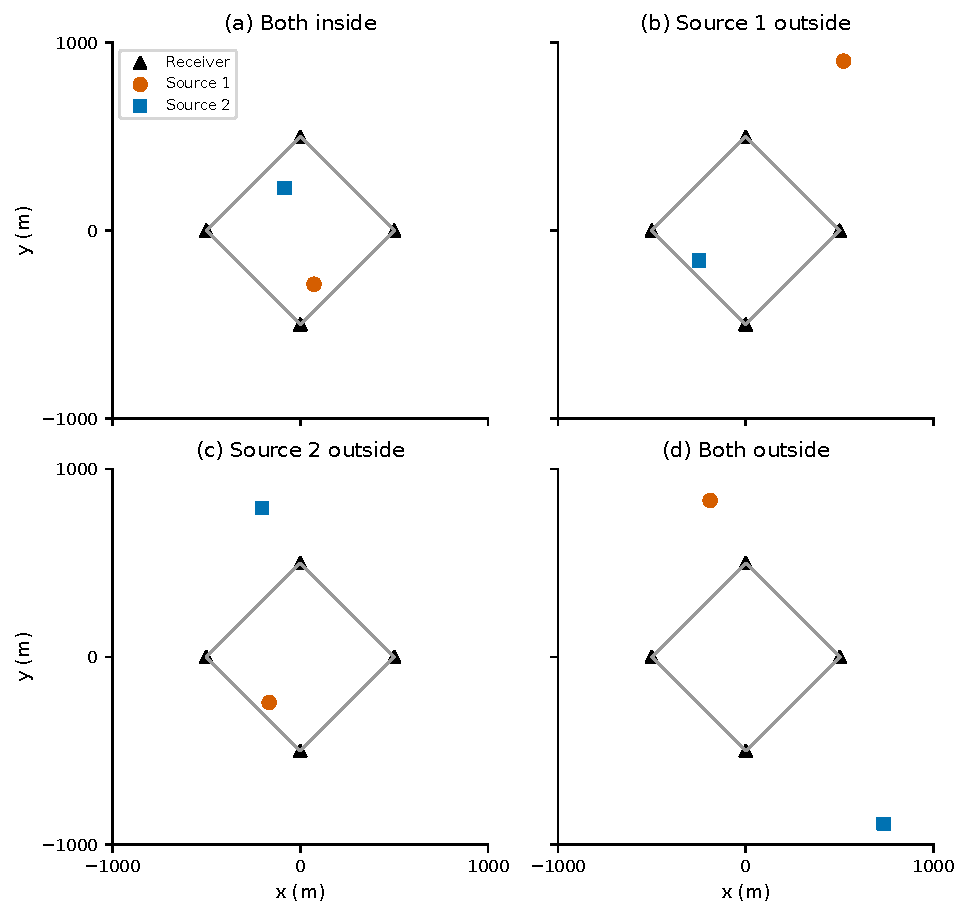
\includegraphics[width=.92\linewidth]{figures/geometry.pdf}
\caption{四类验证布局。三角形为接收站，实线菱形为站点凸包，圆点和方点为源1、源2。四幅图使用相同坐标范围。}\label{fig:geometry}
\end{figure}

\subsection{评价与计时}
设真实集合为$X=\{\bm p_k\}$，估计集合为$Y=\{\widehat{\bm p}_j\}$。成功距离取$r=0.02R=20$\,m。成功率通过门限内的一对一匹配计算：先最大化成功关联数，再最小化其平方距离和。弱源成功率统计源2被有效匹配的比例，双源成功率要求两源均被匹配。同一个估计不能同时计为两个源成功。

未截断误差使用独立的最小平方距离指派。等基数情况下
\begin{equation}
 \pi^*=\arg\min_{\pi}\sum_{k=1}^{K}
 \|\bm p_k-\widehat{\bm p}_{\pi(k)}\|_2^2,\qquad
 e_k=\|\bm p_k-\widehat{\bm p}_{\pi^*(k)}\|_2 .\label{eq:assignment}
\end{equation}
指派用匈牙利算法求解\cite{Kuhn1955}，分别报告强、弱源RMSE以及误差CDF和P95。本文不以成功样本子集计算总体RMSE。

整体集合误差采用GOSPA\cite{Rahmathullah2017}，$p=2$、$c=100$\,m、$\alpha=2$：
\begin{equation}
 d_{\mathrm G}(X,Y)^2=
 \min_{\gamma}\left[\sum_{(k,j)\in\gamma}\|\bm p_k-\widehat{\bm p}_j\|^2
 +\frac{c^2}{2}\left(|X|+|Y|-2|\gamma|\right)\right],\label{eq:gospa}
\end{equation}
其中$\gamma$为一对一部分关联。20\,m是本研究的成功门槛，100\,m是GOSPA截断尺度，二者职责不同。

算法时间从IQ输入后的必要预处理开始，包含DFT、频点筛选、数据传输、搜索、系数求解及精修。GPU运算采用同步计时，公共预热单列。第二组保留求解时间和实验记录开销两个字段，表中使用包含在线轨迹记录的求解墙钟，不含磁盘持久化及事后精度证书。扩大比较将证书成本进一步单列。跨实现比较同时给出运算计数，配对比较则使用相同设备、输入和调用路径。

不确定性按布局内随机实现配对重采样，保留同一波形实现六档功率差的关联。四类固定布局下的区间反映这些布局内的随机变化；扩大几何的统计另行报告。

\subsection{比较方法及可复现配置}\label{sec:baselines}
所有方法共享公共IQ、传播规律、搜索边界和20\,m初始网格。LS、MUSIC和MVDR在各自谱上选峰并进行相应连续精修；AP、多初值与GA求解式\eqref{eq:profile}；SBL使用多频共享稀疏功率。附录\ref{app:baselines}列出其在本场景下的具体准则。表\ref{tab:parameters}给出当前冻结的扩大比较配置；已完成的较早比较采用的差异在对应结果段说明。
\par\begin{table}[htbp]\centering\footnotesize
\caption{扩大比较的冻结方法参数。连续位置优化不受20\,m网格量化。}\label{tab:parameters}
\begin{tabularx}{\linewidth}{@{}p{.18\linewidth}p{.27\linewidth}X@{}}\toprule
版本 & 核心操作 & 参数\\\midrule
LS谱 & 单源LS谱取两个峰 & 共同20 m网格；同谱连续精修\\
MUSIC & 噪声子空间宽带汇聚 & 4段；超噪声功率加权；已知K\\
MVDR-known & 加载协方差逆谱 & 8段；相对加载0.01\\
充分AP & 反复全域条件更新 & 候选5；循环上限6；正常连续精修\\
交替／联合AP & 相同分支，改变精修方式 & 候选1/2/5；每次局部上限100；共同投影梯度阈值$10^{-8}$\\
VP-BNOMP & 残差发现、消元Newton、共同LS & 循环上限200；每次Newton最多5步；步长上限50 m\\
固定系数BNOMP & 原文对应的固定系数更新 & 循环上限10000；能量阈值$10^{-8}$；局部小步阈值0.01 m\\
多初值联合ML & 同一联合LS目标 & 8个唯一初值：4谱峰+4 Sobol；L-BFGS-B\\
GA联合ML & 同一联合LS目标 & 种群128；最多200代；连续30代停滞停止\\
宽带SBL & 共享功率、离网字典、单点$\gamma$ & 最多300轮；每5轮离网更新；8个活动点；原生停止\\
\bottomrule\end{tabularx}\end{table}
\par
扩大比较登记的运行环境为Windows、Python 3.10.20、NumPy 2.2.6和PyTorch 2.8.0+cu129，GPU为NVIDIA GeForce RTX 4070 Ti SUPER，CPU计算线程设为20。响应与目标使用双精度实数／复数运算。
\par

方法实现保留三类区分。频率轴、分段、噪声方差、加载及基本精修属于使方法满足运行条件的常规适配；候选分支和位置更新目标的改变单独列算法版本；批量响应、缓存与小矩阵计算属于公共工程优化。MUSIC采用四段统计及观测超噪声功率加权，MVDR-known采用八段统计与相对加载0.01，均只处理同一物理频带。这里的MVDR-known按式\eqref{eq:mvdr}实现，与DPD-HR的原公式分别命名。

\subsection{混合干扰与逐源处理的作用}
图\ref{fig:gap}给出第一组已完成比较。MUSIC与MVDR-known的孤立弱源20条和孤立强源120条均达到20\,m成功门槛，混合后成功率随功率条件变化明显；AP和VP-BNOMP则在该组120条混合观测中全部成功。孤立源对照排除了“弱源本身普遍不可定位”这一主要解释，也说明联合拟合与逐源处理对本场景具有实际作用。
\begin{figure}[htbp]\centering
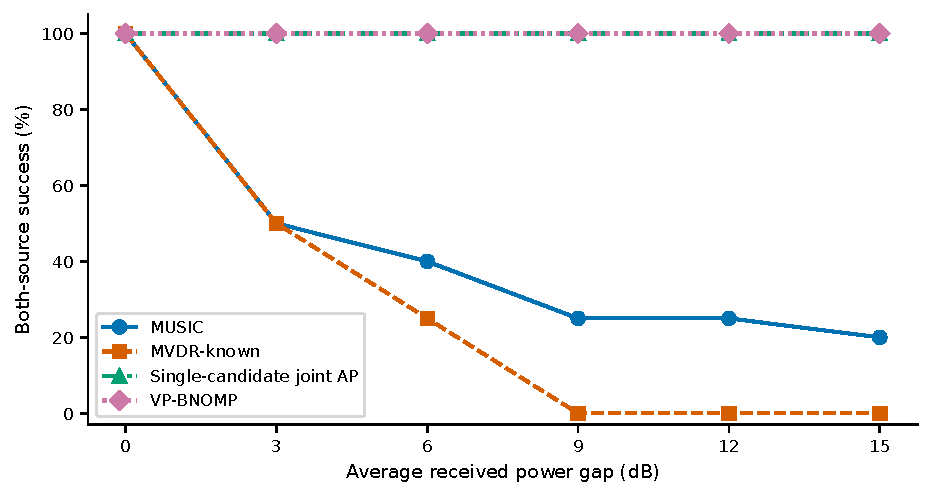
\includegraphics[width=.9\linewidth]{figures/power_gap.pdf}
\caption{已完成带限比较中的双源20\,m成功率。每档20条观测，共120条；每个随机实现的六档功率差共享波形与噪声。图中版本与配置由来源索引逐项登记。}\label{fig:gap}
\end{figure}

这一组比较确立了有竞争力的参照：条件搜索与残差精修能够在本模型下快速处理强弱重叠源。后续实验围绕这些求解器，进一步区分候选恢复和精修成本的收益。

\subsection{候选保留与联合精修的配对结果}\label{sec:apresults}
第二组比较统一初始化与优化精度。单候选交替AP和单候选联合AP均在120条观测中成功110条，位置与最终拟合目标接近；联合精修减少了目标和梯度调用。恢复五候选后，原10条失败全部被正确候选分支恢复。表\ref{tab:paired}给出完整配对结果。
\par\begin{table}[htbp]\centering\small
\caption{相同120条观测的配对结果。RMSE使用全部观测，单位m。}\label{tab:paired}
\begin{tabular}{@{}lrrrrr@{}}\toprule
方法 & 双源成功 & 强源RMSE & 弱源RMSE & GOSPA & 时间/s\\\midrule
单候选交替AP & 110/120 & 0.942 & 103.867 & 10.347 & 0.4071\\
单候选联合AP & 110/120 & 0.942 & 103.866 & 10.347 & 0.3739\\
五候选联合AP & 120/120 & 0.760 & 3.146 & 2.079 & 0.6764\\
VP-BNOMP & 120/120 & 0.761 & 3.146 & 2.078 & 0.5196\\
\bottomrule\end{tabular}\end{table}
\par

\begin{figure}[htbp]\centering
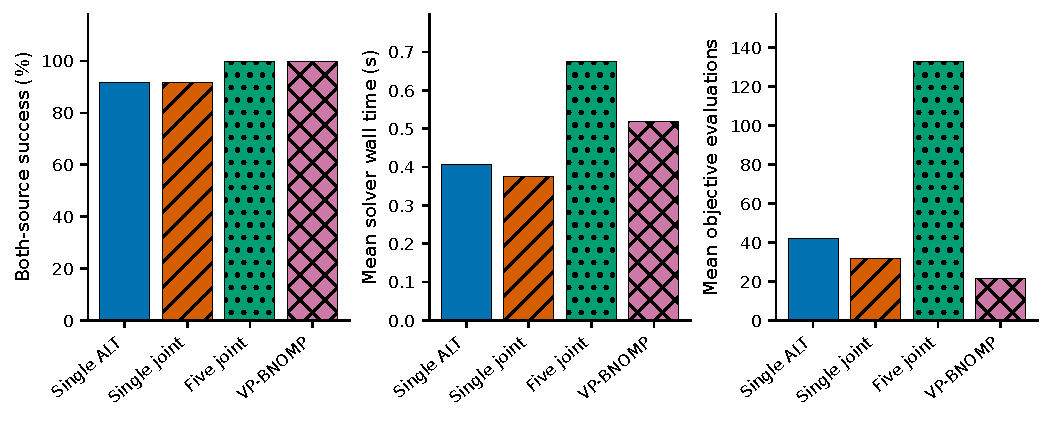
\includegraphics[width=.92\linewidth]{figures/paired_cost.pdf}
\caption{第二组的双源成功率、平均求解墙钟和目标调用次数。前三个AP版本共享输入及共同停止精度；VP-BNOMP保留原生循环停止。五候选成本包括全部分支，不仅统计最终被选分支。}\label{fig:paired}
\end{figure}

单候选联合AP的平均墙钟由0.4071\,s降至0.3739\,s，减少8.15\%；目标调用由41.875次降至31.525次，梯度调用由39.875次降至29.525次。这说明联合精修的主要收益来自计算减少，而非较松的停止条件。五候选联合AP的平均墙钟为0.6764\,s，在增加成本的同时恢复了可靠性。VP-BNOMP平均为0.5196\,s，同样达到120/120成功。两种提出方法在这一组中形成了不同的候选发现和成本取舍。

图\ref{fig:branches}展示多候选发挥作用的一条观测。排名第一的条件候选精修后停留在错误区域，弱源误差为361.21\,m；第二候选精修后误差为0.25\,m，联合残差也更小。两个分支都满足相同精度检验，区别来自进入的局部区域。因而，仅延长第一分支的局部迭代不能替代候选保留。
\begin{figure}[htbp]\centering
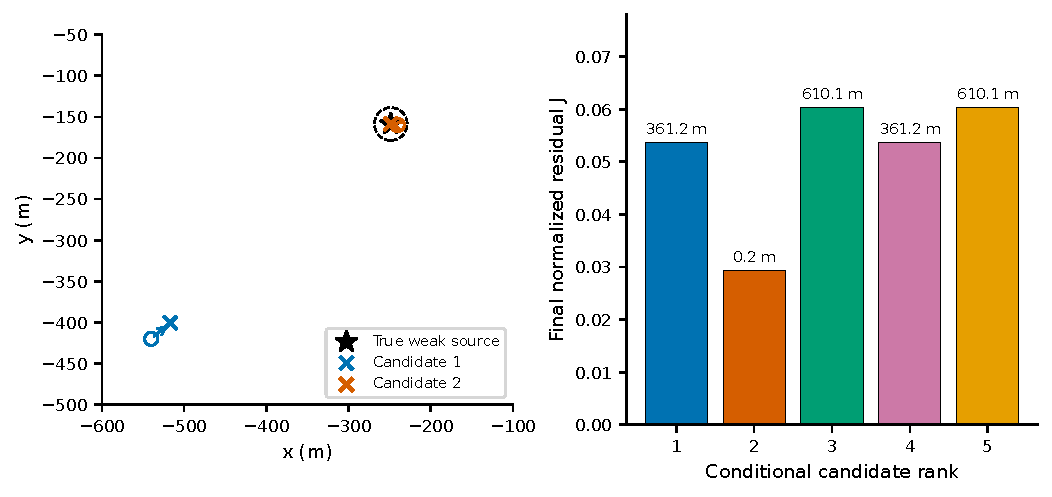
\includegraphics[width=.92\linewidth]{figures/candidate_case.pdf}
\caption{候选恢复案例：源1在站外、源2在站内，功率差6\,dB。左图放大弱源区域，圆圈为候选起点，叉号为精修终点，星号与虚线圆为弱源真值及成功范围；右图使用保存的分支目标与位置误差。该图为事后机制案例，统计结论来自全部120条配对观测。}\label{fig:branches}
\end{figure}

\FloatBarrier
10条恢复观测来自同一个布局中的多个随机实现与功率条件。它们构成候选机制证据；扩大比较将进一步检验这一机制在更多独立几何中的出现频率。图\ref{fig:cdf}保留全部误差，展示成功率之外的长尾变化。
\begin{figure}[htbp]\centering
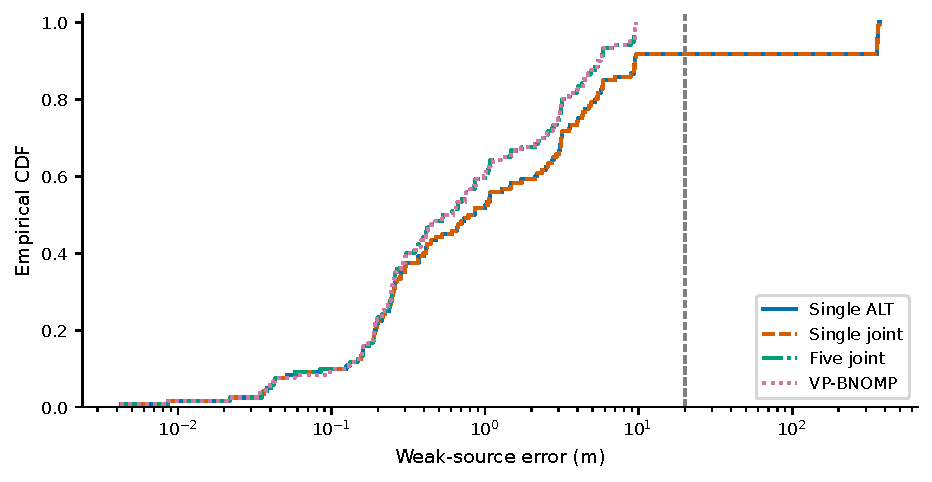
\includegraphics[width=.9\linewidth]{figures/error_cdf.pdf}
\caption{第二组弱源误差CDF，包含全部120条观测；虚线标出20\,m成功门槛。对数横轴展示亚米误差与数百米长尾。}\label{fig:cdf}
\end{figure}

\subsection{固定系数与消元曲率的机制实验}\label{sec:mechanismresults}
为区分停止尺度、数值保护和局部目标的影响，第三组在四个布局、0/15\,dB两档的八条观测上作受控比较。固定系数参照使用原文对应的局部Newton形式、共同系数重估时序和能量停止；消元对照只替换局部位置目标，保留其余时序。另比较放宽能量停止阈值以及取消局部小步长退出，结果见表\ref{tab:mechanism}。
\par\begin{table}[htbp]\centering\small
\caption{八条观测的曲率机制隔离。各行共享相同输入和外层系数更新时序。}\label{tab:mechanism}
\begin{tabular}{@{}lrrrr@{}}\toprule
局部更新与停止 & 双源成功 & 弱源RMSE/m & 时间/s & 导数调用\\\midrule
固定系数，严格停止 & 8/8 & 5.413 & 5.4783 & 2679.500\\
固定系数，阈值$10^{-7}$ & 7/8 & 9.665 & 2.3184 & 1133.875\\
固定系数，阈值$10^{-6}$ & 6/8 & 12.683 & 0.9706 & 467.375\\
固定系数，取消小步退出 & 8/8 & 2.011 & 8.0110 & 4758.375\\
消元更新，严格停止 & 8/8 & 3.221 & 0.4356 & 70.375\\
\bottomrule\end{tabular}\end{table}
\par

\begin{figure}[htbp]\centering
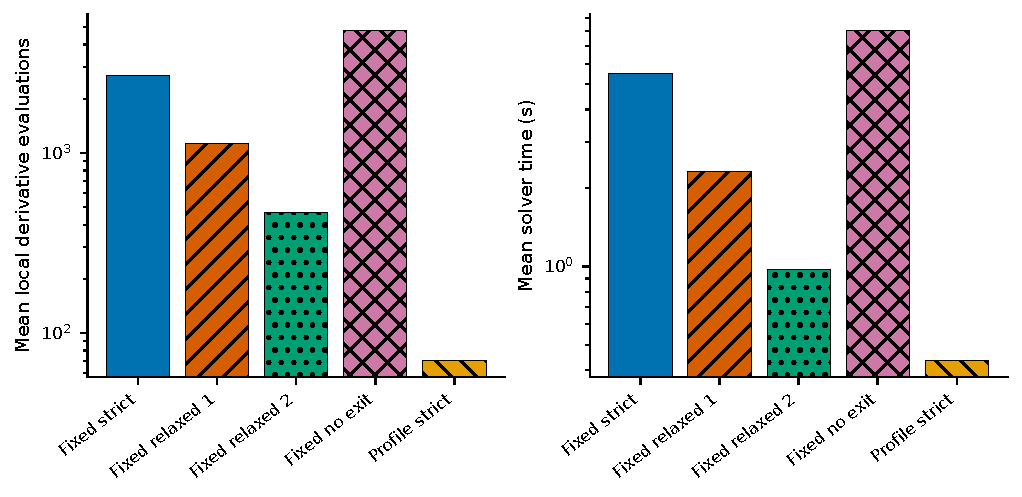
\includegraphics[width=.9\linewidth]{figures/curvature_cost.pdf}
\caption{八条观测的受控曲率实验。左为平均局部导数调用数，右为平均求解时间；纵轴为对数刻度。严格固定系数与严格消元更新共享停止尺度及外层时序。}\label{fig:curvature}
\end{figure}

严格固定系数更新的21436次局部步中，有17935次以已接受的小步触发局部退出，占83.7\%。这组运行未触发Hessian修正、步长截断、边界裁剪或回溯，因而慢收敛主要体现为曲率控制下的反复小步，而非数值保护反复拒绝更新。将能量阈值从$10^{-8}$放宽至$10^{-7}$或$10^{-6}$虽然省时，却降低了20\,m成功数。取消小步退出则增加了计算。

保持严格阈值后，消元更新的平均导数调用从2679.5次降至70.375次，平均时间从5.4783\,s降至0.4356\,s，两者均保持8/8成功。这与式\eqref{eq:schur}所揭示的位置--系数耦合机制一致。该倍率对应八条观测的隔离对照，不作为整套VP-BNOMP在扩大数据上的最终加速比。

\subsection{扩大布局的统一比较}\label{sec:formalpending}
扩大比较已冻结20个布局，四类内外关系各五个布局，每布局20次波形与噪声实现，六档功率差，共2400条混合观测。六个核心版本共享全部2400条输入；八类方法及原文对应BNOMP在共同240条子集上比较，慢方法独立完成后补入同一报告。各阶段保留早期解、最终解、原生停止与实际运算计数。

核心版本包括VP-BNOMP及其末端联合变体、单候选交替AP，以及候选数为1、2、5的联合AP。采用嵌套候选和共同前缀，避免把不同初始化或停止尺度混入部件收益。20个布局中，各类别的前3个用于分析，后2个为锁定验证。正式报告将分别给出分功率差成功率、误差、完整耗时和调用次数，并以布局与随机实现的层次配对统计反映不确定性。

\pending{扩大比较正在运行。本节只登记已经冻结的设置；正式成功率、误差、耗时、区间及方法排名待逐样本审计完成后填入，并据此定稿摘要和结论。}

\section{结论}\label{sec:conclusion}
本文以最小二乘消去未知宽带波形，将同步单天线站的条件搜索、残差发现和联合精修统一到同一位置目标。多候选联合AP保留粗搜索中尚未占优的候选，以精修后的拟合残差择优；波形消元块NOMP保留残差发现和循环更新，通过消元曲率减少位置--信号系数耦合造成的重复小步。

已完成的配对实验表明，候选保留能够恢复单候选的错误区域，联合精修在相同精度要求下减少了目标与梯度调用。受控实验进一步将固定系数更新的慢收敛与曲率机制联系起来，支持以消元目标改善局部更新。两种方法分别从候选可靠性和更新效率出发，为有限观测下的多源直接定位提供了可解释的求解策略。扩大布局的统一比较将用于确定最终性能范围与推荐配置；未知源数及更复杂传播可在这一基础上继续研究。

\clearpage
\begingroup
\small
\setlength{\bibsep}{4pt}
\bibliographystyle{IEEEtranN}
\bibliography{references}
\endgroup
\clearpage
\appendix
\section{比较方法在本模型下的准则}\label{app:baselines}
\subsection{单源谱、MUSIC及MVDR-known}
LS取峰使用式\eqref{eq:single}。对MUSIC和MVDR，将同一记录划分为$S$个不重叠片段，各片段长度为$N_s=N/S$。在片段DFT频率轴上选择相同物理频带，构造
\begin{equation}
 \widehat{\bm C}_f=S^{-1}\sum_{b=1}^S\bm z_{bf}\bm z_{bf}^H .
\end{equation}
统计样本均来自该条观测，不从其他试次借快拍。完整记录与片段DFT分别保持$1/N$和$1/N_s$归一化；其白噪声方差分别为$\sigma_t^2/N$和$\sigma_t^2/N_s$。

设$\bm E_{n,f}$为$\widehat{\bm C}_f$最小$L-K$个特征值对应的特征向量。本文MUSIC适配版使用
\begin{align}
 S_{\mathrm{MU}}(\bm p)&=\left[\sum_f w_f
 \bm q_f(\bm p)^H\bm E_{n,f}\bm E_{n,f}^H\bm q_f(\bm p)\right]^{-1},\label{eq:music}\\
 \widetilde w_f&=\max\{\tr(\widehat{\bm C}_f)-L\sigma_t^2/N_s,0\},\quad
 w_f=\widetilde w_f/\sum_v\widetilde w_v .\nonumber
\end{align}
所有权重为零时退回均匀权重。已知$K$用于划分子空间，$w_f$由观测计算。处理频带外的频点不参与子空间分解。

MVDR-known采用
\begin{align}
 \bm C_{f,\delta}&=\widehat{\bm C}_f+
 \delta\,\tr(\widehat{\bm C}_f)\bm I/L,\nonumber\\
 S_{\mathrm{MV}}(\bm p)&=F_s^{-1}\sum_f
 [\bm q_f(\bm p)^H\bm C_{f,\delta}^{-1}\bm q_f(\bm p)]^{-1} .\label{eq:mvdr}
\end{align}
这里$\delta$为相对加载量，$F_s$为片段频率轴上的有效频点数。“known”表示采用本文已知相对传播响应；命名不等同于原DPD-HR公式的逐项复现。

\subsection{充分AP、多初值联合ML与GA}
充分AP对每个源反复执行全域条件扫描、候选比较及连续精修，更新时采用式\eqref{eq:profile}。它与短流程MCJ-AP共享物理目标，区别在于全域核查和初值处理的次数。完整AP保留早期有效解，因而比较成本时可区分首次可靠输出与最终核查结束。

多初值联合ML从四个唯一的谱峰组合和四个Sobol覆盖组合出发，以有界L-BFGS-B最小化$J$，输出最小残差解。候选组合的无序重复在初始化阶段删除。GA在相同四维位置目标上进行锦标赛选择、模拟二进制交叉和多项式变异\cite{DebAgrawal1995}，保留4个精英，最后作联合连续精修。锦标赛规模为3，交叉概率为0.9、分布指数为15，每维变异概率为0.25、分布指数为20。GA的总体成本由种群、代数和实际目标调用共同决定。

\subsection{多频共享功率SBL}
在公共位置字典$\bm D_f=[\bm q_f(\bm g_1),\ldots,\bm q_f(\bm g_G)]$上，令逐频系数先验为$\bm z_f\sim\mathcal{CN}(0,\bm\Gamma)$，$\bm\Gamma=\diag(\bm\gamma)$跨频共享\cite{Nannuru2019}。于是
\begin{align}
 \bm C_f&=\sigma_f^2\bm I+\bm D_f\bm\Gamma\bm D_f^H,\label{eq:sblCov}\\
 \bm\mu_f&=\bm\Gamma\bm D_f^H\bm C_f^{-1}\bm x_f,\nonumber\\
 \mathcal E(\bm\gamma)&=F^{-1}\sum_f[\log\det\bm C_f+\bm x_f^H\bm C_f^{-1}\bm x_f] .\label{eq:sblEvidence}
\end{align}
平坦频谱先验下，半步固定点更新写为
\begin{equation}
 \gamma_j^+=\gamma_j\left[
 \frac{\sum_f|\bm d_{fj}^H\bm C_f^{-1}\bm x_f|^2}
 {\sum_f\bm d_{fj}^H\bm C_f^{-1}\bm d_{fj}}
 \right]^{1/2} .\label{eq:sblUpdate}
\end{equation}
证据回溯控制更新，每5轮对8个活动字典点作离网优化。每维位移限制为20\,m，坐标尺度为1000\,m，L-BFGS-B最多20轮，最终从单点$\gamma_j$取峰。每5轮检查一次：证据归一化变化小于$10^{-5}$，$\gamma$的L1相对变化小于1\%，输出位置和活动点最大移动均小于0.05\,m；连续两次检查满足时停止，否则最多300轮。谱峰分组候选不并入本文提出方法。

\subsection{局部精修与停止参数}
AP的交替和联合版本在归一化目标$J$上使用相同投影梯度阈值$10^{-8}$，目标差停止项设为零。每次L-BFGS-B最多100轮，线搜索最多25次；交替版本最多12个完整位置扫描。初始化的单源精修采用目标相对容差$10^{-12}$。候选在$3\times3$邻域中取局部极大值，再按30\,m间隔保留；该间隔是候选去重参数，不是成功门槛。

VP-BNOMP每次局部Newton最多5步，Hessian最小特征值下限为$10^{-9}$，位置步长上限为50\,m。按$1,1/2,1/4,1/8,1/16$依次回溯，接受下降步，局部小步阈值为0.01\,m。循环中目标下降小于$10^{-8}$且最大位置移动小于0.05\,m，连续两轮满足时停止。已完成配对组的循环上限为12；扩大比较固定为200，以分别记录原生停止与预算触顶。

\subsection{固定系数BNOMP对应版与消元对照}
原文对应版根据给定系数$q_f^{(0)}$使用
\begin{equation}
 L_{\mathrm{FC}}(\bm p)=E_x^{-1}\sum_f
 \|\bm y_f-\bm a_f(\bm p)q_f^{(0)}\|^2 .\label{eq:fixedcoef}
\end{equation}
对位置求Newton方向，再按该版的时序重估系数。本文以二维多频块NOMP\cite{Yang2022}为对应来源，移植的是系数固定下的位置更新及循环结构，观测由声学波束形成改为本研究的四站时延--幅度响应。符号、单位、边界和数值保护均按本模型登记。

受控消元版只把式\eqref{eq:fixedcoef}改成式\eqref{eq:localprofile}，用于隔离曲率效应；VP-BNOMP还采用其自身的共同系数重估时序。受控版的倍率与完整算法的对比结果分开报告，避免把多个时序差异都归于一处。

\section{消元局部导数与实现核验}\label{app:derivatives}
令$\kappa=2\pi f/c_0$，$\ell_l=\log a_l=-\log d_l-\mathrm j\kappa d_l$。在远离站点的区域，
\begin{align}
 \nabla\ell_l&=(-d_l^{-1}-\mathrm j\kappa)\bm v_l,\\
 \nabla^2\ell_l&=d_l^{-2}\bm v_l\bm v_l^T
 +\frac{-d_l^{-1}-\mathrm j\kappa}{d_l}
 (\bm I-\bm v_l\bm v_l^T),\\
 \nabla^2 a_l&=a_l[\nabla^2\ell_l+(\nabla\ell_l)(\nabla\ell_l)^T].\label{eq:responseHessian}
\end{align}
对固定的$\bm y_f$，将$q_f$拆为实部和虚部，其系数Hessian为
\begin{equation}
 H_{uu,f}=2\|\bm a_f\|^2\bm I_2/E_x .
\end{equation}
逐频计算混合导数并累加Schur补，即可得到式\eqref{eq:localprofile}的$2\times2$实Hessian。实现核验分别对照直接最小二乘、投影消元、解析梯度、有限差分和小规模直接矩阵。理论恒等式核验与定位性能实验分别记录。

\end{document}
